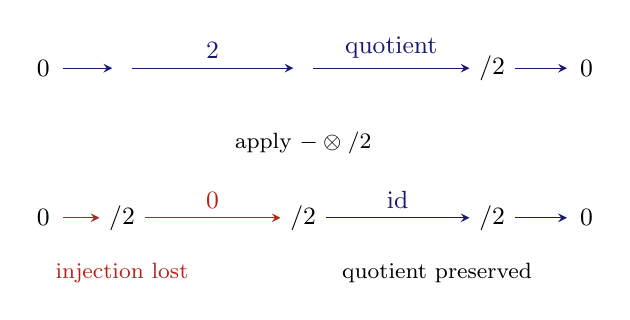
\begin{tikzpicture}[x=1cm,y=1cm,>=stealth, every node/.style={font=\small}]
\node at (0,1.3) {$0$};
\node (a) at (1,1.3) {$\Z$};
\node (b) at (3.3,1.3) {$\Z$};
\node (c) at (5.7,1.3) {$\Z/2$};
\node at (6.9,1.3) {$0$};
\draw[->,MidnightBlue] (0.25,1.3)--(a);
\draw[->,MidnightBlue] (a)--node[above] {$2$}(b);
\draw[->,MidnightBlue] (b)--node[above] {quotient}(c);
\draw[->,MidnightBlue] (c)--(6.65,1.3);
\node at (0,-0.6) {$0$};
\node (d) at (1,-0.6) {$\Z/2$};
\node (e) at (3.3,-0.6) {$\Z/2$};
\node (f) at (5.7,-0.6) {$\Z/2$};
\node at (6.9,-0.6) {$0$};
\draw[->,BrickRed] (0.25,-0.6)--(d);
\draw[->,BrickRed] (d)--node[above] {$0$}(e);
\draw[->,MidnightBlue] (e)--node[above] {$\mathrm{id}$}(f);
\draw[->,MidnightBlue] (f)--(6.65,-0.6);
\node[font=\footnotesize,align=center] at (3.3,0.35) {apply $-\otimes_{\Z}\Z/2$};
\node[font=\footnotesize,text=BrickRed] at (1,-1.3) {injection lost};
\node[font=\footnotesize] at (5,-1.3) {quotient preserved};
\end{tikzpicture}
